\documentclass[border=4pt]{standalone}
\usepackage{amsmath,amssymb,amsfonts}
\usepackage{xcolor,colortbl,array,booktabs,multirow}
\usepackage{tikz}
\usepackage{pgfplots}
\pgfplotsset{compat=1.16}
\usetikzlibrary{arrows, automata, backgrounds, calendar, chains, decorations,
    matrix, mindmap, patterns, petri, positioning, shadows, shapes.geometric,
    trees, shapes, decorations.pathreplacing, calc, tikzmark, arrows.meta,
    intersections, fit, graphs, quotes, angles, decorations.markings}
\newcommand{\st}{\text{ s.t. }}
\newcommand{\x}{\mathbf{x}}
\renewcommand{\b}{\mathbf{b}}
\renewcommand{\c}{\mathbf{c}}
\newcommand{\A}{\mathbf{A}}
\newcommand{\y}{\mathbf{y}}
\newcommand{\z}{\mathbf{z}}
\newcommand{\R}{\mathbb{R}}
\newcommand{\RR}{\mathbb{R}}
\newcommand{\Z}{\mathbb{Z}}
\newcommand{\ZZ}{\mathbb{Z}}
\newcommand{\npcomplete}{NP-complete}
\providecommand{\true}{\text{TRUE}}
\providecommand{\false}{\text{FALSE}}
\tikzset{vertex/.style={circle,fill=black!25,minimum size=20pt,inner sep=0pt},
    edge/.style={draw,thick,-},weight/.style={font=\small},
    selected vertex/.style={vertex, fill=red!24},
    selected edge/.style={draw,line width=2pt,-,red!50},
    ignored edge/.style={draw,line width=2pt,-,black!20}}
\newcommand{\vect}{\vec}
\providecommand{\ds}{\displaystyle}
\providecommand{\longvect}{\overrightarrow}
\usepackage[normalem]{ulem}
\definecolor{ocre}{RGB}{243,102,25}
\providecommand{\leftB}{\left[}
\providecommand{\rightB}{\right]}
\tikzset{directed/.style={postaction={decorate,decoration={markings,mark=at position .65 with {\arrow{>}}}}},
    directed1/.style={postaction={decorate,decoration={markings,mark=at position .65 with {\arrow{>}}}}}}
\begin{document}
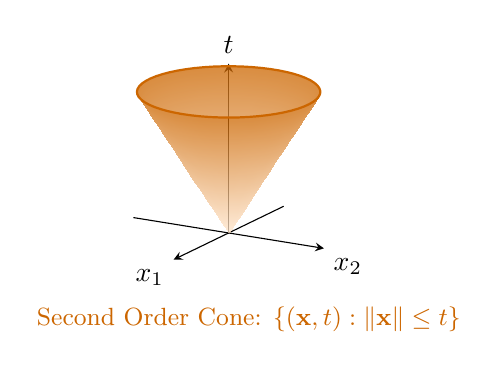
\begin{tikzpicture}
% Second Order Cone in R^3: ||(x1,x2)|| <= t
% compat set locally: the book preamble has no \pgfplotsset{compat=...},
% and old-compat axis label placement scatters t/x2 across the page.
\pgfplotsset{compat=1.16}
\begin{axis}[
    width=5.4cm, height=4.8cm,
    view={120}{20},
    axis lines=center,
    ticks=none,
    xlabel={$x_1$}, ylabel={$x_2$}, zlabel={$t$},
    xlabel style={anchor=north east},
    ylabel style={anchor=north west},
    zlabel style={anchor=south},
    zmin=0, zmax=1.2,
    xmin=-1.2, xmax=1.2, ymin=-1.2, ymax=1.2,
    clip=false]
  % lateral surface of the cone t = ||(x1,x2)||
  \addplot3[surf, shader=interp,
      colormap={soc}{color=(orange!20) color=(orange!80!black)},
      opacity=0.75, domain=0:1, y domain=0:360,
      samples=14, samples y=40, z buffer=sort]
      ({x*cos(y)}, {x*sin(y)}, {x});
  % rim of the cone at t = 1
  \addplot3[orange!80!black, thick, domain=0:360, samples=60]
      ({cos(x)}, {sin(x)}, {1});
\end{axis}
\node[orange!80!black, below=1pt] at (current bounding box.south)
    {\small Second Order Cone: $\{(\x, t) : \|\x\| \leq t\}$};
\end{tikzpicture}
\end{document}
